\documentclass[10pt]{beamer}

\usetheme[progressbar=frametitle]{metropolis}
\usepackage{appendixnumberbeamer}

\usepackage{booktabs}
\usepackage[scale=2]{ccicons}
\usepackage{listings}
% % \usetheme[progressbar=frametitle]{metropolis}
\usepackage{appendixnumberbeamer}
\usepackage[utf8]{vietnam}
\usepackage[utf8]{inputenc}
\usepackage[vietnamese]{babel}
\usepackage[T1]{fontenc}
%\renewcommand\sfdefault{cmbr}
\usepackage{booktabs}
\usepackage[scale=2]{ccicons}
\usepackage{ragged2e}
\apptocmd{\frame}{}{\justifying}{}
\usepackage{pgfplots}
\usepgfplotslibrary{dateplot}
\usepackage[upright]{fourier}
\usepackage{tikz}



\usetikzlibrary{matrix,arrows,decorations.pathmorphing}


\definecolor{rosy}{RGB}{247, 215, 148}
\definecolor{summer}{RGB}{245, 205, 121}
\definecolor{beige}{RGB}{253, 227, 167}
\definecolor{sblack}{RGB}{64, 64, 64}
\setbeamercolor{frametitle}{bg=rosy,%bg=beige,
fg=sblack}

\usepackage{hyperref}
\hypersetup{
    colorlinks=true,
    linktoc=all,
    linkcolor=black,
}
\usepackage{relsize}
\usepackage{textpos}
\addtobeamertemplate{frametitle}{}{%
\begin{textblock*}{100mm}(\textwidth,-1.05cm)
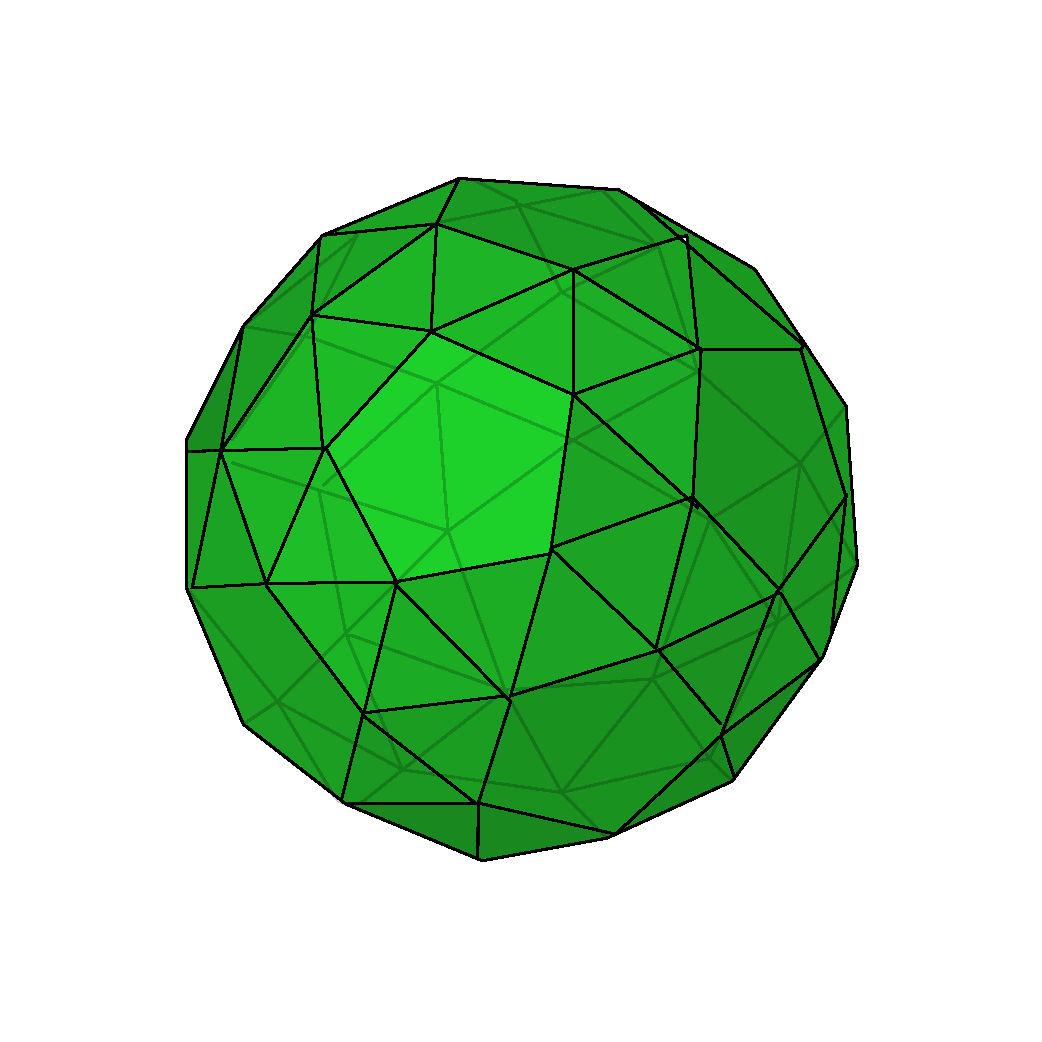
\includegraphics[height=1cm,width=1cm,keepaspectratio]{logo.pdf}
\end{textblock*}}

\usepackage{xspace}

\setbeamerfont{page number in head/foot}{size=\tiny}
\setbeamercolor{footline}{fg=gray}
\setbeamertemplate{frame footer}{}

% \newcommand{\themename}{\textbf{\textsc{metropolis}}\xspace}
\usepackage{cmbright}

\usepackage{pgfplots}
\usepgfplotslibrary{dateplot}

\usepackage{xspace}
\newcommand{\themename}{\textbf{\textsc{metropolis}}\xspace}
\usepackage{xparse}

\NewDocumentCommand{\codeword}{v}{%
\texttt{\textcolor{blue}{#1}}%
}

\lstset{language=tex,keywordstyle={\bfseries \color{blue}}}

\title{Vim Workshop}
\subtitle{CSHub 2019}
\date{\today}
\date{}
\author{Tien Phan (attacker0211)}
\institute{York University, Toronto, Canada}
%\titlegraphic{\hfill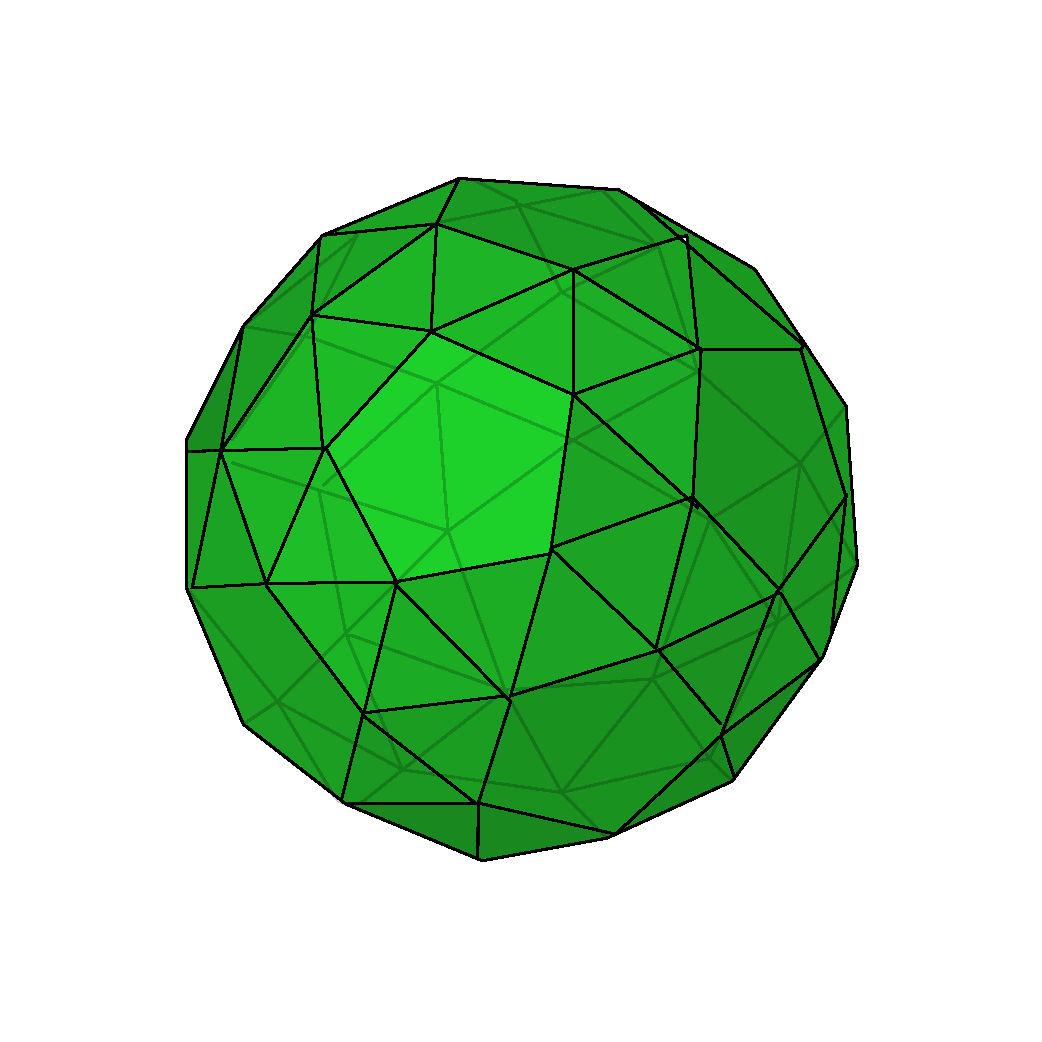
\includegraphics[height=1.5cm]{logo.pdf}}

\begin{document}

\maketitle

\begin{frame}{Contents}
  \setbeamertemplate{section in toc}[sections numbered]
  \tableofcontents[hideallsubsections]
\end{frame}


\section{Introduction to Vim}

\begin{frame}{Vim Installation}
https://www.vim.org/download.php
% \begin{itemize}
%   \item
% \end{itemize}
\end{frame}

\begin{frame}{Vim???}
\begin{itemize}
  \item<1-> Vim is a highly configurable text editor for efficiently creating, changing, replacing any kind of text.
  \item<2-> It is included as "vi" in most Unix systems.
  \item<3-> Many other editors such as Visual Studio Code supports vim emulation mode.
  \item<3-> Vim is worth learning even if you finally end up switching to some other text editor.
\end{itemize}
\end{frame}

\begin{frame}{Why Vim?}
  
\includegraphics[width=200pt]{vimi.jpg}
\end{frame}

\begin{frame}{Why Vim?}
  \begin{itemize}
    \item<1-> Vim is a modal editor with different modes for manipulating text:
    \begin{itemize}
      \item \textbf{Normal mode} - used for editor commands. This is also the default mode.
      \item \textbf{Visual mode} - similar to normal mode, but used to highlight areas of text. Normal commands are run on the highlighted area, which for an instance can be used to move or edit a selection.
      \item \textbf{Select mode} - works similarly to visual mode. However, if a printable character, carriage return, or newline (or line feed) is entered, Vim inserts the character, and starts insert mode.
      \item \textbf{Insert mode} - similar to editing in most modern editors.
      \item  \textbf{Command-line mode} - supports a single line input at the bottom of the Vim window. Normal commands (beginning with :), and some other specific letters corresponding to different actions (including pattern search and the filter command) activate this mode.
      \item \textbf{Ex mode}, it takes a single line input at the bottom of the window.
    \end{itemize}
  \end{itemize}
\end{frame}

\begin{frame}{Why Vim?}
  \begin{itemize}
    \item<1->Vim avoid the use of the mouse because it's too slow, and even avoid arrow keys because it requires too much movement.
    \item<2->Vim is programmable with Vimscript and Vim commands are composable.
    \item<3->Vim operates at the speed speed of thought
    \item<4->And so much more crazier stuff, seriously. I'm still learning Vim everyday.
  \end{itemize}
\end{frame}

\section{Basics}
\begin{frame}{Insert/Insert Mode}
  \begin{itemize}
    \item From normal mode, press \textbf{i/a/o} to enter insert mode. Press \textbf{ESC} to return to normal mode.
  \end{itemize}
\end{frame}

\begin{frame}{Command Mode/Normal Mode}
  
\includegraphics[width=200pt]{vim-exit.jpg}
\end{frame}

\begin{frame}{Command Mode}
  \begin{itemize}
    \item \textbf{:q} quit
    \item \textbf{:w} save
    \item \textbf{:e} open for editing
    \item \textbf{:help}
    \item \textbf{:\%s/find/replace}
  \end{itemize}
\end{frame}

\begin{frame}{Movements}
\begin{itemize}
  \item Basic movement: hjkl (left, down, up, right)
  \item Words: w (next word), b (beginning of word), e (end of word)
  \item Lines: 0 (beginning of line), \^ (first non-blank character), \$ (end of line)
  \item Screen: H (top of screen), M (middle of screen), L (bottom of screen)
  \item Scroll: Ctrl-u (up), Ctrl-d (down)
  \item File: gg (beginning of file), G (end of file)
  \item Line numbers: \{number\}G
  \item Find: f{character}, t\{character\}, F\{character\}, T\{character\}
  find/to forward/backward \{character\} on the current line
  \item Search: /\{findMatch\}, n / N for next / previous matches
\end{itemize}
\end{frame}

\begin{frame}{Edits}
\begin{itemize}
  \item \textbf{d\{motion\}} delete \{motion\}
  e.g. dw is delete word, d\$ is delete to end of line, d0 is delete to beginning of line
  \item \textbf{c\{motion\}} change \{motion\}
  e.g. cw is change word
  like d{motion} followed by i
  \item \textbf{x} delete character (equal do dl)
  \item \textbf{s} substitute character (equal to xi)
  \item visual mode + manipulation
  select text, d to delete it or c to change it
  \item \textbf{u} to undo, \textbf{$<$C-r$>$} to redo
  \item \textbf{y} to copy /“yank” (some other commands like \textbf{d} also copy)
  \item \textbf{p} to paste
\end{itemize}
\end{frame}

\begin{frame}{Edits}
  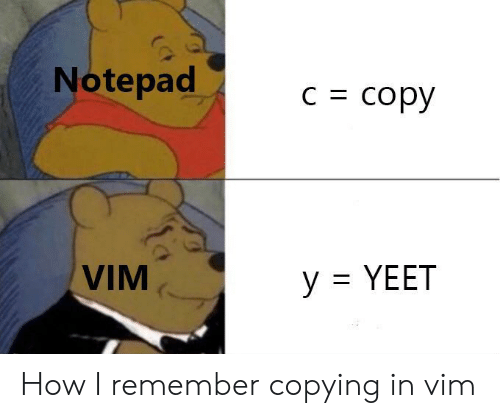
\includegraphics[width=220pt]{yank.png}
\end{frame}

\begin{frame}{Visual Mode}
  \begin{itemize}
    \item Character mode: \textbf{v} (lower-case)
    \item Line mode: V (upper-case)
    \item Block mode: Ctrl+v
  \end{itemize}

\end{frame}

\begin{frame}{Modifier}
\begin{itemize}
  \item ci( :change the contents inside the current pair of parentheses
  \item ci[ :change the contents inside the current pair of square brackets
  \item da' :delete a single-quoted string, including the surrounding single quotes
\end{itemize}
\end{frame}

\begin{frame}{Ex Mode}
  \begin{itemize}
    \item Takes a single line input at the bottom of the window.
    \item However, in Cmdline mode, entering a command exits the mode when the command is executed. Entering a command in Ex mode doesn't cause the mode to change.
  \end{itemize}
\end{frame}

\section{Advances}
\begin{frame}{Macros}
  \begin{itemize}
    \item Start recording by pressing q, followed by a lower case character to name the macro.
    \item Perform any typical editing, actions inside Vim editor, which will be recorded.
    \item Stop recording by pressing q.
    \item Play the recorded macro by pressing $@$ followed by the macro name.
    \item To repeat macros multiple times, press: number$@$macro-name.
  \end{itemize}
\end{frame}

\begin{frame}{Search and replace}
\begin{itemize}
  \item :s (substitute) command

  \item \%s/foo/bar/g: replace foo with bar globally in file
\end{itemize}
\end{frame}

\begin{frame}{Windows/Tab/Buffer}
  \begin{itemize}
    \item \textbf{Multiple windows:} :sp / :vsp to split windows
    \item Vim maintains a set of open files, called “buffers”.
    \item A Vim session has a number of tabs, each of which has a number of windows (split panes). \\
    :tabnew to create a new tab.
    \item Can have multiple views of the same buffer.
  \end{itemize}
\end{frame}

\section{Configure Vim Yourself!}
\begin{frame}{Configuring Vim}
  \begin{itemize}
    \item<1-> The configuration file should be in ~/.vimrc
    \item<2-> I recommend start with someone else's dotfiles first. When I first started, I used: https://github.com/thoughtbot/dotfiles
  \end{itemize}
\end{frame}

\begin{frame}{Plugins}
  \begin{itemize}
    \item Some famous plugin managers: Pathogen(https://github.com/tpope/vim-pathogen/), Vundle (https://github.com/VundleVim/Vundle.vim).
    \item nerdtree (file explorer): https://github.com/preservim/nerdtree
    \item ctrlp.vim (fuzzy file finder): https://github.com/ctrlpvim/ctrlp.vim
    \item nerdcommenter: https://github.com/preservim/nerdcommenter
    \item vim-autoclose (auto close brackets): https://github.com/Townk/vim-autoclose
    \item vim-surround (surroundings everything): https://github.com/tpope/vim-surround
    \item UltiSnips (for snippets): https://github.com/SirVer/ultisnips
  \end{itemize}
\end{frame}


\section{Resources}
\begin{frame}{Resources}
  \begin{itemize}
    \item vimtutor
    \item \href{https://vim.fandom.com/wiki/Vim_Tips_Wiki}{Vim Wiki}
  \end{itemize}
\end{frame}
\end{document}
